\documentclass[10pt,a4paper]{article}
\usepackage[margin=2.2cm]{geometry}
\usepackage[T1]{fontenc}
\usepackage{lmodern,microtype,amsmath,graphicx,booktabs,array,xcolor,tabularx,multirow,enumitem}
\usepackage{listings}
\usepackage{tikz}
\usetikzlibrary{positioning,arrows.meta,fit}
\usepackage[colorlinks,linkcolor=blue!50!black,urlcolor=blue!50!black,citecolor=blue!50!black]{hyperref}
\lstset{basicstyle=\ttfamily\footnotesize,columns=fullflexible,keepspaces,frame=single,framerule=0.3pt,
  rulecolor=\color{black!30},backgroundcolor=\color{black!3},breaklines,showstringspaces=false,
  commentstyle=\color{black!55},morecomment=[l]{\#},xleftmargin=2pt,xrightmargin=2pt}
\newcommand{\code}[1]{\texttt{\detokenize{#1}}}
\newcommand{\hMsun}{$h^{-1}M_\odot$}
\setlist{itemsep=1pt,topsep=3pt}
\title{The Sahyadri pkdgrav3 pipeline on pawna:\\ setup, bugs fixed, and systematic tests of the halo catalogs}
\author{Sahyadri collaboration --- prepared with Claude Code}
\date{11 November 2026 \\[2pt] \small repository \code{a-paranjape/sahyadri-sandbox}, branch \code{rockstar-pkc-reader}}

\begin{document}
\maketitle

\begin{abstract}
We describe the end-to-end pipeline that runs a Sahyadri simulation on the pawna cluster: pkdgrav3 writing
compressed \code{.pkc} snapshots, Rockstar reading them directly, consistent-trees, value-added catalogs
(\code{.vahc}, \code{.tens}) and conversion to FITS, submitted as a chain of PBS jobs from one configuration file.
We list the bugs found and fixed on the way, three of which change or blocked existing data products, and report
systematic tests of the different ways of producing a halo catalog from the same simulation: the native
\code{.pkc} reader, the same particles converted to Gadget format, the uncompressed (raw) pkdgrav3 particles,
a 4\% particle subsample, and repeated runs. With one reader the \code{.pkc} route reproduces the Gadget route
byte for byte. Compression changes halo counts, masses, $V_{\max}$, positions and velocities at the per-mille level
without bias; the inner structure (scale radius, spin) of halos with fewer than $\sim$1000 particles is the most
sensitive. Wall time and peak memory of every stage are measured for $128^3$ and $512^3$ runs. All figures are
made by a notebook from data files kept in the repository.
\end{abstract}

\tableofcontents

%======================================================================
\section{Overview}
\label{sec:overview}

\begin{figure}[h]
\centering
\begin{tikzpicture}[node distance=4mm and 7mm, every node/.style={font=\footnotesize},
  st/.style={draw,rounded corners,fill=blue!6,align=center,minimum height=12mm,text width=24mm},
  da/.style={align=center,text width=26mm,font=\scriptsize\ttfamily},
  ar/.style={-{Stealth[length=2mm]},thick}]
\node[st] (sim) {\textbf{sim}\\pkdgrav3\\\code{job_sim.pbs}};
\node[st,right=of sim] (rs) {\textbf{rockstar}\\Rockstar (PKC)\\\code{job_rockstar.pbs}};
\node[st,right=of rs] (ct) {\textbf{ctrees}\\consistent-trees\\\code{job_ctrees.pbs}};
\node[st,right=of ct] (va) {\textbf{vahc}\\\code{run_addvalue.py}\\\code{job_vahc.pbs}};
\node[st,right=of va] (fi) {\textbf{fits}\\\code{compress_halo_outputs}\\\code{job_fits.pbs}};
\foreach \a/\b in {sim/rs,rs/ct,ct/va,va/fi} \draw[ar] (\a) -- node[above,font=\scriptsize]{afterok} (\b);
\node[da,below=of sim] {snap.<step>.s<pct>.<w>.pkc\\snapnames.txt};
\node[da,below=of rs] {out_<snap>.list\\halos_<snap>.*};
\node[da,below=of ct] {out_<snap>.trees\\trees/, scales.txt};
\node[da,below=of va] {out_<snap>.vahc\\out_<snap>.tens};
\node[da,below=of fi] {compressed/*.fits.gz\\+ check log};
\draw[ar,dashed,black!50] (sim.north) to[bend left=18] node[above,font=\scriptsize]{particles (.pkc subsamples) read again} (va.north);
\end{tikzpicture}
\caption{The five stages, each a PBS job started only if the previous one succeeded (\code{afterok}). One bash
configuration file describes a run; \code{submit_pipeline.sh} submits the chain.}
\label{fig:pipeline}
\end{figure}

The stages and what each needs are listed in Table~\ref{tab:stages}. The scripts are in
\code{scripts/pkdgrav3_pipeline/}; the step-by-step guide (setup, all options, troubleshooting) is
\code{docs/pkdgrav3_pipeline_pawna.md}, and the design and validation notes of the Rockstar reader are in
\code{docs/rockstar_pkc_reader_plan.md}. This report summarises both and adds the systematic tests and
resource measurements.

\begin{table}[h]
\centering\footnotesize
\begin{tabularx}{\textwidth}{@{}l l X X@{}}
\toprule
Stage & Code (version) & Reads & Writes \\
\midrule
sim & pkdgrav3, \code{shadaba/pkdgrav3} \code{main} & config $\to$ \code{p.par}, transfer function & \code{.pkc} files per output, subsample and writer; \code{snapnames.txt}; \code{pkc_check} per output \\
rockstar & Rockstar \code{36ce9eea36ee} + Sahyadri files (PKC reader, curvature, $w_0$--$w_a$) & \code{.pkc} (\code{FILE_FORMAT = "PKC"}); cosmology from the headers & \code{out_<snap>.list}, \code{halos_<snap>.*}, \code{rockstar.cfg} \\
ctrees & consistent-trees \code{7c20add} + Sahyadri background patch; \code{clean_trees.pl} & all \code{out_<snap>.list} & \code{out_<snap>.trees} (hlists), \code{trees/}, \code{../scales.txt}, configs in \code{logs/} \\
vahc & \code{scripts/post-process/run_addvalue.py} (\code{AddValue}) & particles (CIC density), \code{out_<snap>.trees} & \code{out_<snap>.vahc} ($b_1$, tidal and Hessian eigenvalues), \code{out_<snap>.tens} \\
fits & \code{compress_halo_outputs.py}, \code{check_compressed_halos.py} & \code{.trees}, \code{.vahc}, \code{.tens}, \code{trees/} & \code{compressed/*.fits.gz} with cosmology and run metadata; column-by-column check \\
\bottomrule
\end{tabularx}
\caption{Pipeline stages. The order is forced: \code{.vahc}/\code{.tens} rows are the halos of
\code{out_<snap>.trees} (consistent-trees IDs), and the FITS stage folds $b_1$ into the basic catalog and may delete
the ASCII files.}
\label{tab:stages}
\end{table}

%======================================================================
\section{Setting up and running the pipeline}
\label{sec:running}

\subsection{Dependencies and one-time setup}
Everything is built as the user, in directories on \code{/storage}; nothing needs root.
\begin{description}[leftmargin=0pt]
\item[pkdgrav3] with the compressed output, built by pkdgrav3's own \code{tools/pawna/setup_pawna.sh}
  (GCC 11, CMake 3.22, OpenMPI 5 module, HDF5 1.10, GSL, FFTW 3, Boost from the system; zstd, cpptrace and
  libdwarf fetched by CMake). It also provides \code{pkc_check}, \code{pkc_to_gadget} and the zstd library
  that Rockstar links against.
\item[Halo codes and Python] \code{scripts/pkdgrav3_pipeline/setup_pawna.sh <CODES> [PKD_IO_ROOT]} clones
  Rockstar (bitbucket, \code{36ce9eea36ee}) and consistent-trees (\code{7c20add}), copies the changed files kept
  in this repository under \code{code/} over them, builds Rockstar with \code{make with_hdf5_pkc}, builds
  consistent-trees, creates a self-contained Python venv (numpy, scipy, pandas, h5py, fitsio, zstandard; the
  system scipy on pawna needs numpy $<1.25$) and compiles the C helpers of the post-processing
  (\code{cic_update.so}, \code{ngp_update.so}). It took 40 minutes on the pawna login node, 37 of them pip
  building packages from source.
\end{description}

\begin{lstlisting}[language=bash]
# pkdgrav3 (once, 20-40 min)
git clone -b main https://github.com/shadaba/pkdgrav3.git /tmp/$USER-pkd-setup
bash /tmp/$USER-pkd-setup/tools/pawna/setup_pawna.sh /storage/$USER/pkdgrav3_io
# this repository + Rockstar + consistent-trees + Python (once, ~40 min)
git clone -b rockstar-pkc-reader https://github.com/a-paranjape/sahyadri-sandbox.git
bash sahyadri-sandbox/scripts/pkdgrav3_pipeline/setup_pawna.sh /storage/$USER/sahyadri_codes /storage/$USER/pkdgrav3_io
\end{lstlisting}

\subsection{One configuration file per run}
A run is described by a bash \code{KEY=VALUE} file (\code{example_512.conf}, \code{example_test128.conf}):
paths (\code{SANDBOX}, \code{PKD_IO_ROOT}, \code{CODES}, \code{SCRATCH}, \code{LOGS}); run identity
(\code{STEM}, \code{REAL}, \code{NPART}, \code{LBOX}, \code{SEED}); cosmology (including $w_0$, $w_a$ and
$\Omega_{\rm DE}$); output redshifts and time steps; snapshot format (\code{.pkc} subsample percents, optional
HDF5); per-stage cores, memory and wall time; Rockstar settings (readers, writers, \code{FORCE_RES} defaulting to
the pkdgrav3 softening $L/N/50$, minimum halo sizes, \code{PKC_SUBSAMPLES}); tree cleaning; grid, downsampling and
parallelism of the value-added step; FITS options. Every job sources the same file, so a run is reproducible from it.

\subsection{Submission, chaining and restarts}
\begin{lstlisting}[language=bash]
P=sahyadri-sandbox/scripts/pkdgrav3_pipeline
$P/submit_pipeline.sh my.conf --dry-run        # print the qsub commands
$P/submit_pipeline.sh my.conf                  # sim -> rockstar -> ctrees -> vahc -> fits (afterok chain)
$P/submit_pipeline.sh my.conf --stages sim     # only the simulation now ...
$P/submit_pipeline.sh my.conf --stages rockstar,ctrees,vahc,fits --after 2536500.pawna   # ... the rest after it
$P/submit_pipeline.sh my.conf --hold           # first job held; qrls <id> starts the chain
for r in 1 2 3 4 5; do                         # realisations: one config (and one chain) each
  sed "s/^REAL=.*/REAL=$r/; s/^SEED=.*/SEED=$((1000+r))/" my.conf > my_r$r.conf; $P/submit_pipeline.sh my_r$r.conf
done
\end{lstlisting}
Each job writes its own log, \code{$LOGS/<stage>.<run>.<jobid>.log} (PBS's copy-back is unreliable on pawna), and a
memory record \code{<...>.mem.tsv} (Section~\ref{sec:resources}). If a stage fails, PBS removes the jobs that
depend on it; after fixing the cause the chain is resubmitted from that stage with \code{--stages}. The vahc and fits
stages skip finished snapshots and write under temporary names; sim, rockstar and ctrees start over
(Rockstar can resume from its \code{restart.cfg} with \code{RS_RESTART=1}). Any stage also runs without PBS, e.g.\
\code{CONF=$PWD/my.conf PIPE_ENV=$P/pipeline_env.sh STAGE=vahc bash $P/job_vahc.pbs}.

\subsection{Directory layout}
Outputs follow the layout the post-processing (\code{readers.py}) expects: \code{$SCRATCH/sims/<STEM>/r<REAL>/}
(parameter file, \code{.pkc} snapshots, \code{snapnames.txt}, logs), \code{$SCRATCH/halos/<STEM>/r<REAL>/}
(Rockstar, consistent-trees, \code{.vahc}, \code{.tens}, \code{compressed/}) and
\code{$SCRATCH/halos/<STEM>/scales.txt}. \code{snapnames.txt} maps Rockstar's snapshot number to pkdgrav3's step.
For the value-added step only the \code{.pkc} subsamples selected by \code{PP_DOWN_TO} are read; with
\code{PP_DOWN_TO=512} at $2048^3$ these are the 1\% and 3\% files, so keeping them (4\% of the snapshot volume)
is enough to recompute \code{.vahc}/\code{.tens} later.

%======================================================================
\section{The compressed snapshot format and its precision}
\label{sec:pkc}
pkdgrav3 writes each output as \code{.pkc} files: particles are split into random subsamples (by default
1, 3, 5, 9, 10, 12, 15, 20, 25\%), and within each file positions are stored as integers on a grid of
\code{ncell}$\times$\code{sub} steps per box side and velocities in steps of \code{vel_step}, then entropy coded
with zstd. For the $512^3$, $50\,h^{-1}$Mpc validation run the header gives \code{ncell} $=512$, \code{sub} $=50$:
a position step of $50/(512\cdot50)=1.953\,h^{-1}$kpc, equal to the force softening $L/N/50$, and a velocity step
of $2.44$ km/s, about 10 bytes per particle. Figure~\ref{fig:quant} compares the particles of the 1\% subsample at
$z=0$ with pkdgrav3's raw (single precision, uncompressed HDF5) output of the same step: the errors are uniform
within half a step, as expected for rounding.

\begin{figure}[h]\centering
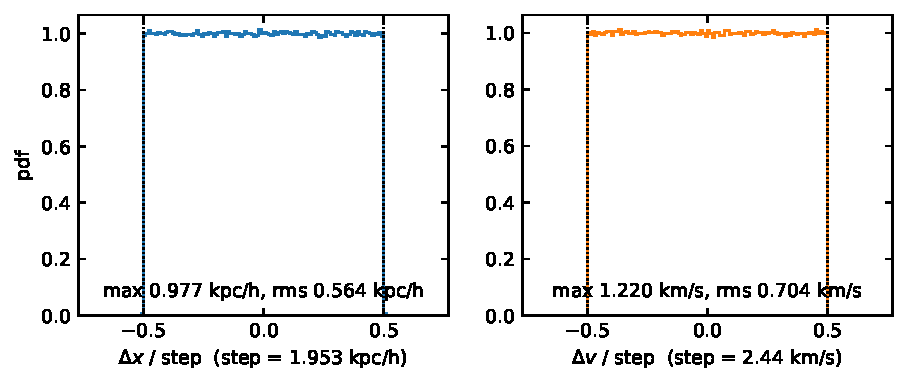
\includegraphics[width=0.75\textwidth]{figures/quantization.pdf}
\caption{Per-particle difference between \code{.pkc} and the raw HDF5 output ($512^3$, $z=0$, 1\% subsample),
in units of the quantization step. Dotted: $\pm$ half a step.}
\label{fig:quant}
\end{figure}

%======================================================================
\section{Bugs found and fixed}
\label{sec:bugs}
Table~\ref{tab:bugs} lists the problems found while building and testing the pipeline. The first three affect
data products that already exist or could not be made with the code in the repository.

\begin{table}[h]
\centering\footnotesize
\begin{tabularx}{\textwidth}{@{}>{\raggedright}p{3.4cm} X >{\raggedright\arraybackslash}p{3.6cm}@{}}
\toprule
Where & Problem and effect & Fix \\
\midrule
\code{correlations.density_hessian_field} & Smoothed the caller's Fourier-space density in place. \code{add_value} computes the Hessian at 3 then 5\,$h^{-1}$Mpc, so \textbf{\code{lamH1/2/3_R5Mpch} in every existing \code{.vahc}} came from a field smoothed twice (3 and 5\,$h^{-1}$Mpc Gaussians); \code{.tens} computed after a \code{.vahc} in the same process were affected the same way. On the $128^3$ test the old values have 0.55--0.63 of the correct rms (Fig.~\ref{fig:vahc}); every other column is unchanged. & Work on a copy (as \code{tidal_tensor_field} already did). \\
\code{correlations.halobyhalo_b1} & Raised ``Please specify number density nbar'' since commit \code{e77922b} (Feb 2026): \code{.vahc} could not be produced with the repository code. & \code{nbar=inf} (no shot-noise subtraction, as in the production code); output byte-identical to production. \\
\code{postprocess.py} (repository version) & Sorted halos by mass before \code{add_value}, so \code{.vahc} rows did not follow \code{.trees}; production (\code{sorthalos=False}) did not. & Keep file order; add \code{add_tens}; the FITS converter refuses misaligned files. \\
\code{readers.read_block} & \code{down_to} was dead code after an early return: all particles were read and used; files not closed. & Downsampling restored; files closed. \\
\code{cic_update.c} (production copy on pegasus) & Particle count passed as \code{int}: overflow above $2^{31}$ particles (production stayed below with \code{down_to=512}). & Repository version uses \code{long}. \\
consistent-trees (upstream) & Flat $\Lambda$CDM everywhere: time table from $\Omega_m$ only, $\Delta_{\rm vir}$ with a cosmological constant, $w_0$/$w_a$ in \code{merger_tree.cfg} ignored. Affects every curved or $w_0$--$w_a$ run (times, accretion rates, consistency step). & Background $E(a)$ as in Rockstar's \code{hubble.c}, in C and Perl; flat $\Lambda$CDM byte-identical to upstream. \\
\code{gen_merger_cfg.pl} & $w_0$, $w_a$ for consistent-trees taken from the hand-written Rockstar input config, not from the catalogs. & Read from a \code{\#w0} line Rockstar now prints (only for non-$\Lambda$CDM). \\
Rockstar & Not deterministic: \code{srand(getpid())} and particle arrival order with several readers. & Not changed; a fixed-seed test build is used for exact tests only. \\
Pipeline (pawna) & PBS \code{-o} copy-back unreliable; system scipy incompatible with current numpy; HDF5 file locking hangs h5py on \code{/storage} (NFS). & Jobs write their own logs; self-contained venv; \code{HDF5_USE_FILE_LOCKING=FALSE}. \\
\bottomrule
\end{tabularx}
\caption{Bugs and problems found, their effect and the fix (details in \code{docs/pkdgrav3_pipeline_pawna.md},
Section 7, and \code{docs/rockstar_pkc_reader_plan.md}).}
\label{tab:bugs}
\end{table}

\begin{figure}[h]\centering
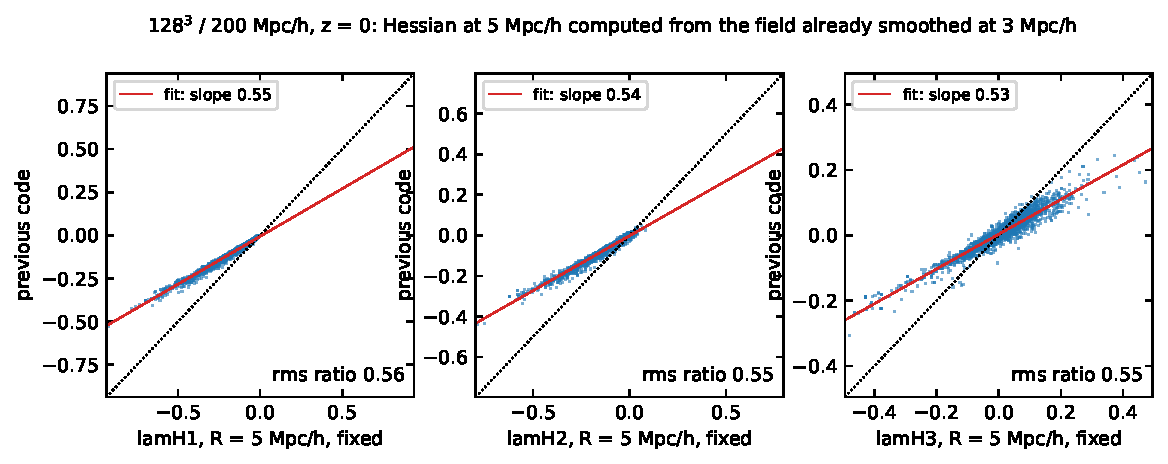
\includegraphics[width=\textwidth]{figures/vahc_bug.pdf}
\caption{Density-Hessian eigenvalues at $R=5\,h^{-1}$Mpc for the 4736 halos of the $128^3$/$200\,h^{-1}$Mpc test
at $z=0$: previous code against the fixed code. The previous values are a strongly smoothed version of the correct
ones.}
\label{fig:vahc}
\end{figure}

%======================================================================
\section{Systematic tests: different ways of making the halo catalog}
\label{sec:routes}

\subsection{Set-up}
One pkdgrav3 run, $512^3$ particles in $50\,h^{-1}$Mpc ($m_p = 8.11\times10^7$\,\hMsun, flat $\Lambda$CDM,
outputs at $z=3,2,1,0.5,0.25,0$), was written both as \code{.pkc} (default precision) and as standard HDF5. Rockstar
(same binary and settings, 8 readers and 8 writers, \code{FORCE_RES} $=1.95\,h^{-1}$kpc, \code{MIN_HALO_OUTPUT_SIZE} $=20$)
was run on the inputs of Table~\ref{tab:routes}, all six outputs in one invocation (temporal halo finding on).

\begin{table}[h]
\centering\footnotesize
\begin{tabularx}{\textwidth}{@{}l X@{}}
\toprule
Route & Input to Rockstar \\
\midrule
\code{pkc} & the \code{.pkc} files, native reader (\code{FILE_FORMAT = "PKC"}) --- the pipeline's route \\
\code{pkc2} & the same, run again: Rockstar's own run-to-run scatter (the noise floor) \\
\code{gad} & the same quantized particles converted to Gadget-2 by \code{pkc_to_gadget --blocks 8} \\
\code{h5g} (``raw'') & pkdgrav3's uncompressed HDF5 output of the same steps, converted to Gadget-2 (\code{--from-hdf5}) \\
\code{pkcsub} & native reader on the 1\% and 3\% subsamples only (\code{PKC_SUBSAMPLES = "1,3"}): a quick-look option, particle mass $\times 25$ \\
\code{pkc1}, \code{gad1} & $z=0$ only, one reader, fixed-seed test build: exactness of the reader \\
\bottomrule
\end{tabularx}
\caption{Rockstar input routes compared.}
\label{tab:routes}
\end{table}

Halos of \code{out_<snap>.list} were matched between two routes by nearest centre (periodic KD-tree), within
$10\,h^{-1}$kpc below $M_{\rm vir}=10^{12}$\,\hMsun\ and $50\,h^{-1}$kpc above. A matched pair whose masses differ by
more than 50\% is a host/subhalo assignment ``flip''; flips are counted but excluded from the medians.

\subsection{Exactness of the reader}
With one reader and the fixed seed, \code{pkc1} and \code{gad1} give byte-identical \code{out_0.list},
\code{halos_<snap>.0.ascii} and \code{halos_<snap>.0.bin} (\EXACT). The native reader therefore hands Rockstar exactly
the particles, masses and header values that the Gadget route does. With 8 readers the catalogs of \code{pkc} and
\code{gad} differ, but only as much as two \code{pkc} runs differ from each other (Fig.~\ref{fig:matched}): what
remains is Rockstar's dependence on the order in which particles reach the writers.

\subsection{Effect of compression: raw particles vs \code{.pkc}}
\begin{figure}[p]\centering
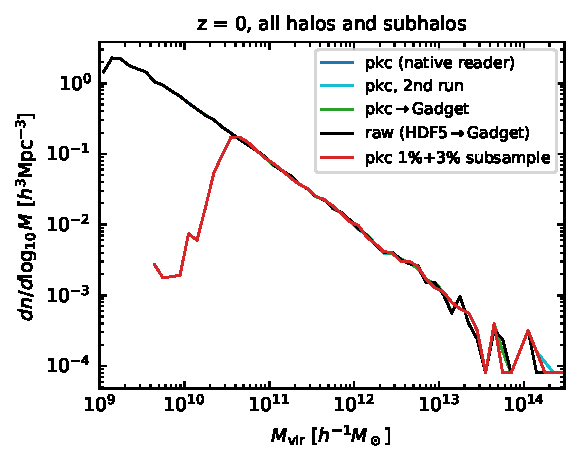
\includegraphics[width=0.43\textwidth]{figures/massfunction.pdf}\\[2mm]
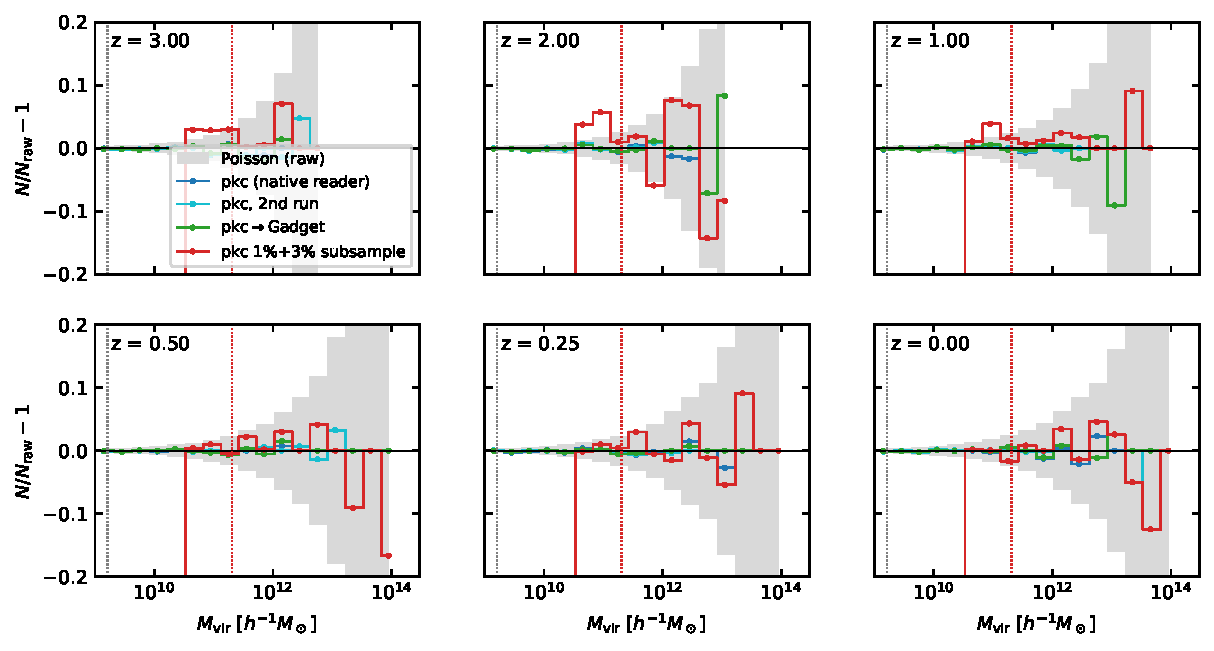
\includegraphics[width=\textwidth]{figures/massfunction_ratio.pdf}
\caption{Top: mass function at $z=0$ for each route. Bottom: ratio to the raw-particle route at every output;
grey band: Poisson error of the raw counts; grey dotted line: 20 particles; red dotted line: 100 particles of the
subsample route.}
\label{fig:mf}
\end{figure}
\begin{figure}[p]\centering
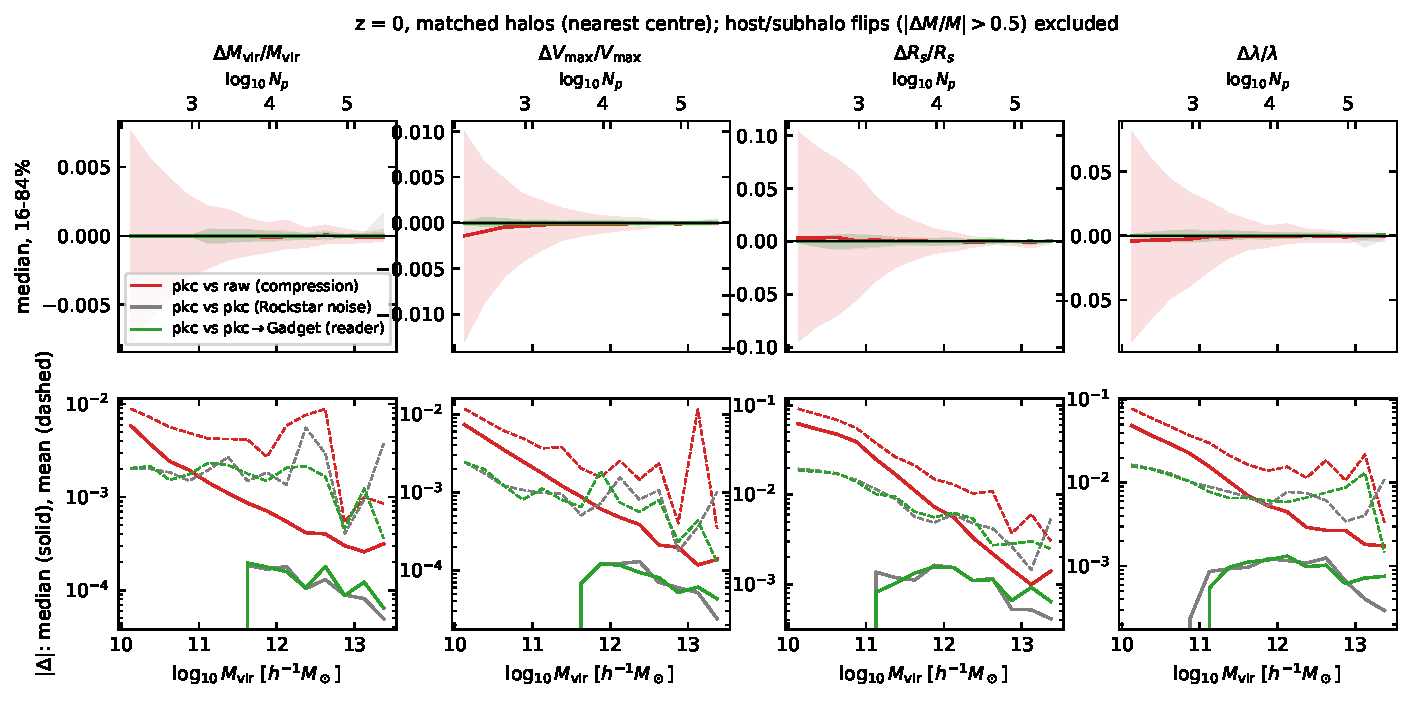
\includegraphics[width=\textwidth]{figures/matched_z0.pdf}
\caption{Differences between matched halos at $z=0$ as a function of mass (top axis: number of particles). Top
row: median and 16--84\% range of the signed relative difference; bottom row: median absolute difference. Red:
\code{.pkc} vs raw particles (effect of compression); grey: two runs on the same \code{.pkc} input (Rockstar
noise); green: native reader vs the same particles in Gadget format.}
\label{fig:matched}
\end{figure}

\begin{table}[h]
\centering\scriptsize\setlength{\tabcolsep}{3pt}
\begin{tabular}{@{}l r r r r r r r r r r@{}}
\toprule
$\log_{10}M_{\rm vir}$ & $N$ & $N/N_{\rm raw}-1$ [\%] & matched [\%] & flips [\%] & med $\Delta M/M$ & med $|\Delta M/M|$ & med $|\Delta V_{\max}/V_{\max}|$ & centre [kpc/$h$] & $|\Delta R_s/R_s|$ [\%], bias & $|\Delta\lambda/\lambda|$ [\%], bias \\
\midrule
$10$--$11$ & 31764 & -0.00 (0.6) & 99.50 (99.92) & 0.9 (0.2) & 0 & 3.9e-3 (0) & 5.1e-3 (0) & 0.86 (0.00) & 5.52 (0.00), +0.42 & 3.80 (0.00), -0.31 \\
$11$--$12$ & 4213 & -0.12 (1.5) & 99.69 (99.93) & 1.3 (0.2) & 0 & 1.1e-3 (0) & 1.2e-3 (6.0e-5) & 0.64 (0.03) & 1.73 (0.13), +0.07 & 1.09 (0.10), -0.06 \\
$12$--$13$ & 510 & -0.20 (4.4) & 99.80 (100.00) & 3.9 (1.0) & 0 & 4.5e-4 (1.4e-4) & 3.4e-4 (1.1e-4) & 0.66 (0.16) & 0.36 (0.12), -0.02 & 0.33 (0.11), -0.04 \\
$13$--$15$ & 57 & +1.79 (13.4) & 100.00 (100.00) & 5.3 (1.8) & -7.7e-5 & 2.7e-4 (8.7e-5) & 1.3e-4 (5.7e-5) & 0.87 (0.33) & 0.11 (0.05), -0.03 & 0.15 (0.04), -0.01 \\

\bottomrule
\end{tabular}
\caption{Compression effect at $z=0$ (\code{pkc} vs raw), in mass bins of $10^{10}$--$10^{11}$ (123--1230 particles)
up to $>10^{13}$\,\hMsun; in brackets the same quantity for \code{pkc} vs \code{pkc2} (Rockstar noise) or, for
$N/N_{\rm raw}-1$, the Poisson error. Medians over matched halos without flips. Generated by the notebook.}
\label{tab:compression}
\end{table}

\COMPRESSIONTEXT

\begin{figure}[h]\centering
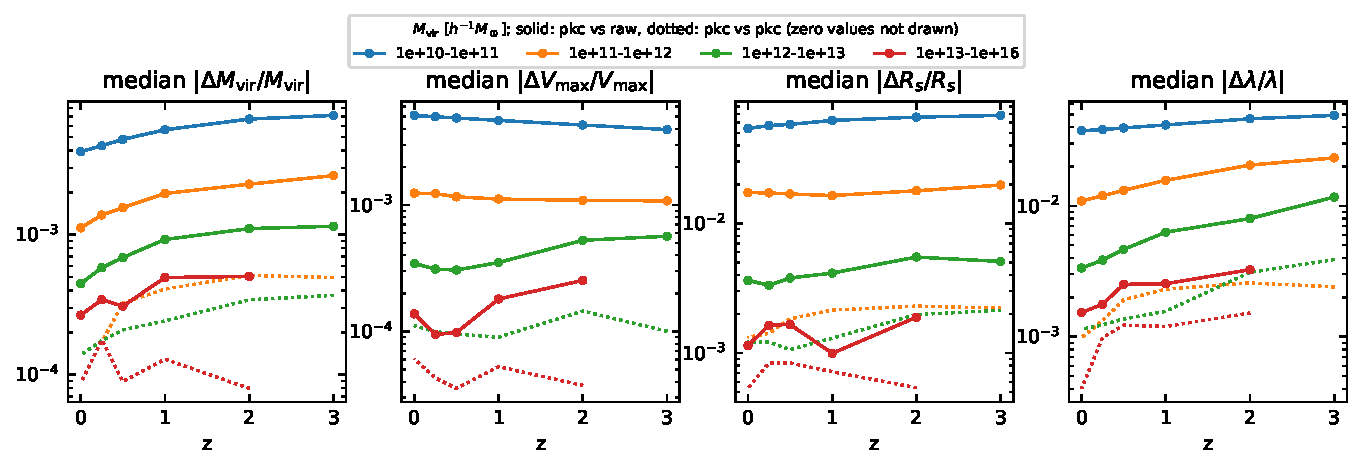
\includegraphics[width=\textwidth]{figures/redshift_dependence.pdf}
\caption{Median absolute difference vs redshift in four mass bins. Solid: \code{.pkc} vs raw; dotted: \code{pkc}
vs \code{pkc2} (values of exactly zero are drawn at $10^{-6}$).}
\label{fig:zdep}
\end{figure}
\begin{figure}[h]\centering
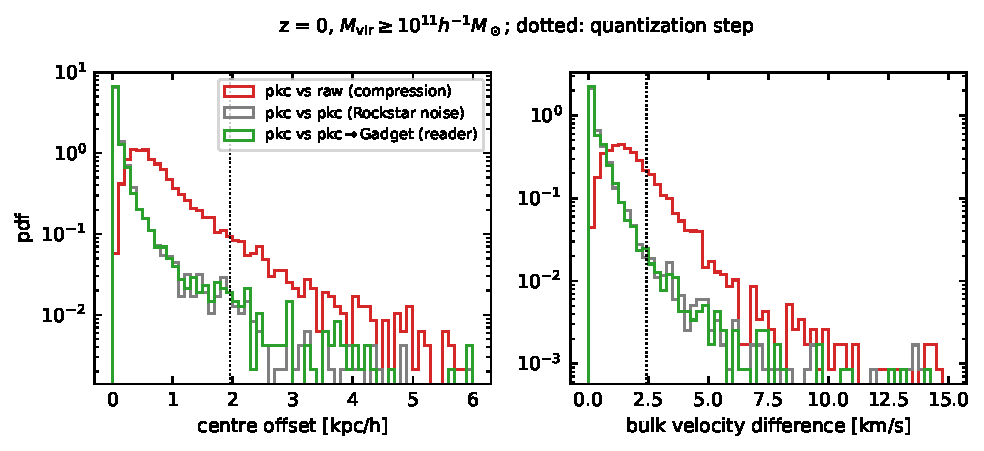
\includegraphics[width=0.8\textwidth]{figures/offsets.pdf}
\caption{Distribution of centre offsets and bulk-velocity differences of matched halos with
$M_{\rm vir}\geq10^{11}$\,\hMsun\ at $z=0$.}
\label{fig:offsets}
\end{figure}

\subsection{Halo finding on a 4\% subsample}
\SUBSAMPLETEXT

\subsection{Merger trees}
\CTREESTEXT

%======================================================================
\section{Wall time and memory}
\label{sec:resources}
pawna puts every PBS job into the same cgroup (\code{/system.slice/pbs.service}), so the kernel keeps no per-job
memory peak, and PBS's own accounting was not kept after the jobs ended. Every pipeline job therefore runs
\code{memmon.sh}, which every 5\,s (2\,s for the validation steps) sums over the job's process tree the
proportional set size (PSS: a page shared by $n$ processes counts $1/n$ in each, so the sum is the memory really
occupied) and the resident set size (RSS, shared pages counted in every process: an upper bound). Peaks shorter than
the sampling interval can be missed. The monitor was checked on the login node against two processes allocating
2\,GB and 1\,GB (measured 3.04\,GB PSS).

\RESOURCETEXT

\begin{table}[h]
\centering\footnotesize
\begin{minipage}[t]{0.52\textwidth}\centering
\begin{tabular}{@{}l l r r r r@{}}
\toprule
Run & Stage & Wall [s] & PSS [GB] & RSS [GB] & proc. \\
\midrule
512$^3$ & sim & 4780 & 25.09 & 25.10 & 4 \\
512$^3$ & rockstar & 475 & 8.03 & 8.22 & 27 \\
512$^3$ & ctrees & 506 & 0.80 & 0.91 & 9 \\
512$^3$ & vahc & 3666 & 91.56 & 91.74 & 9 \\
512$^3$ & fits & 153 & 5.90 & 5.90 & 2 \\
128$^3$ & sim & 110 & 5.86 & 5.88 & 4 \\
128$^3$ & rockstar & 41 & 0.20 & 0.38 & 27 \\
128$^3$ & ctrees & 9 & 0.00 & 0.01 & 2 \\
128$^3$ & vahc & 49 & 2.29 & 2.52 & 10 \\
128$^3$ & fits & 6 & 0.10 & 0.11 & 2 \\

\bottomrule
\end{tabular}
\end{minipage}\hfill
\begin{minipage}[t]{0.45\textwidth}\centering
\begin{tabular}{@{}l r r r r@{}}
\toprule
Step ($512^3$ validation) & Wall [s] & PSS [GB] & RSS [GB] & halos $z{=}0$ \\
\midrule
pkc & 803 & 8.33 & 8.86 & 239939 \\
pkc2 & 849 & 8.35 & 8.88 & 239965 \\
gad & 818 & 8.25 & 8.78 & 239946 \\
h5g & 815 & 8.23 & 8.75 & 239973 \\
pkc1 & 764 & 6.53 & 6.54 & 239997 \\
gad1 & 798 & 6.53 & 6.54 & 239997 \\
pkcsub & 105 & 0.84 & 0.95 & 15851 \\
convert & 388 & 10.04 & 10.05 & -- \\
ctrees pkc & 643 & 1.44 & 1.44 & -- \\
ctrees h5g & 452 & 1.43 & 1.44 & -- \\

\bottomrule
\end{tabular}
\end{minipage}
\caption{Left: pipeline stages for the $128^3$ and $512^3$ runs (both $200\,h^{-1}$Mpc). Right: Rockstar input routes
and other steps of the $512^3$/$50\,h^{-1}$Mpc validation (6 outputs; \code{pkc1}/\code{gad1}: $z=0$ only).
PSS and RSS are peaks of the sum over the job's processes; ``proc.'' is the number of processes at the PSS peak.}
\label{tab:resources}
\end{table}

\begin{figure}[h]\centering
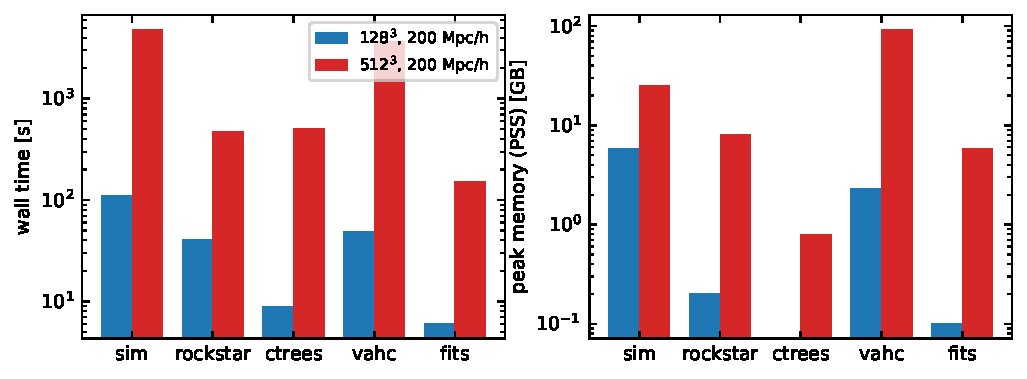
\includegraphics[width=0.8\textwidth]{figures/stages_resources.pdf}\\
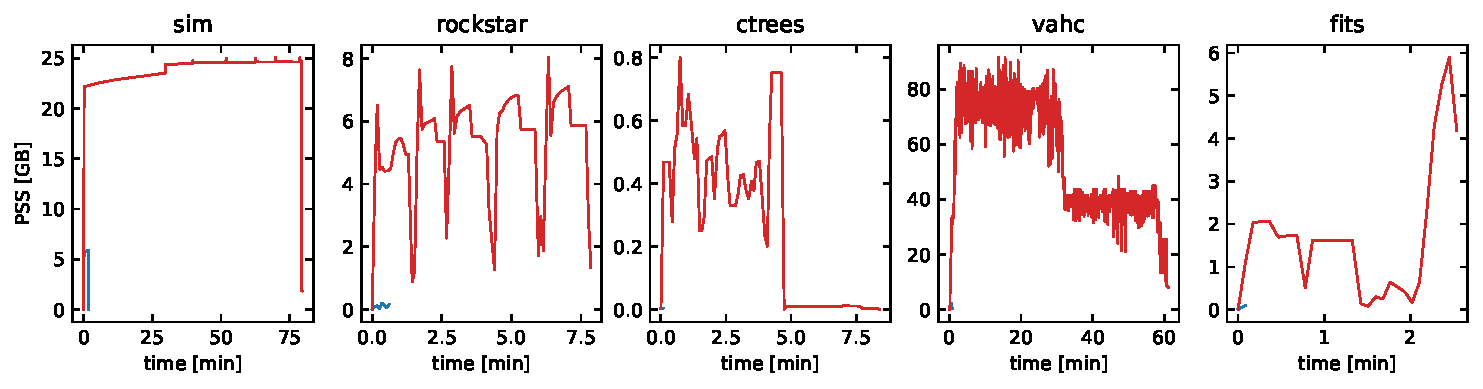
\includegraphics[width=\textwidth]{figures/memory_timeline.pdf}\\
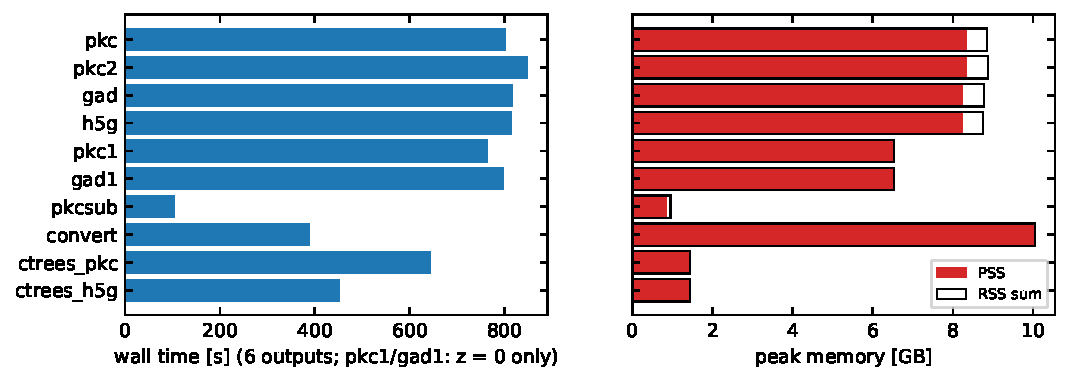
\includegraphics[width=0.8\textwidth]{figures/routes_resources.pdf}
\caption{Top: wall time and peak memory per pipeline stage. Middle: memory (PSS) during each stage. Bottom: Rockstar
input routes and other validation steps at $512^3$.}
\label{fig:resources}
\end{figure}

%======================================================================
\section{Caveats and open questions}
\begin{itemize}
\item Nothing above $512^3$ has been run. Rockstar memory at $2048^3$ (64 times the particles) is extrapolated, not
  measured; whether one pawna node (755\,GB) suffices must be tested at $1024^3$ first.
\item Rockstar's particle mass constant ($\rho_{\rm crit}=2.77519737\times10^{11}$) differs from the one used by
  \code{pkc_to_gadget} and the PKC reader ($2.77536627\times10^{11}$) by $6\times10^{-5}$; Sahyadri should pick one.
\item Rockstar treats radiation as curvature; consistent-trees' \code{clean_trees.pl} matches hlists by five
  characters of the scale factor, so outputs closer than $\Delta a=0.001$ would collide.
\item The \code{.vahc} files on pegasus have wrong \code{lamH*_R5Mpch} columns (Section~\ref{sec:bugs}) and should be
  regenerated (the 1\% and 3\% \code{.pkc} subsamples, or the downsampled Gadget particles, suffice).
\end{itemize}

%======================================================================
\section{Reproducing this report}
\begin{itemize}
\item \code{docs/report/extract_data.py} (with \code{extract_job.pbs}) reduces the pawna catalogs and logs to the
  files in \code{docs/report/data/}.
\item \code{docs/report/make_figures.ipynb} makes every figure and the generated tables from those files only
  (\code{build_notebook.py} holds its source).
\item Validation jobs: \code{scripts/rockstar/pkc_validation/} (\code{run_val512.pbs}, \code{rockstar_val.pbs},
  \code{compare_*.py}); pipeline runs: \code{scripts/pkdgrav3_pipeline/} with the configurations given in the text.
\end{itemize}

\end{document}
